The data specification of trajectory-return pairs distinguishes our empirical study from most existing works in offline RL. Omitting step-wise rewards naturally increases the challenges in decision-making.

\subsection{Overview}
% Here we report the dataset, the tasks and the numbers...
Our empirical study adopts the convention from offline RL. We first train our model with the offline data and then test it as an agent in the corresponding task. More training details and ablation studies of LPT can be found in~\cref{appen:training,appen:ablation}.

\textbf{OpenAI Gym-Mujoco} The D4RL offline RL dataset \citep{fu2020d4rl} features densely-rewarded locomotion tasks including {\em Halfcheetah, Hopper}, and {\em Walker2D}. We test for {\em medium} and {\em medium-replay}. 
It also includes {\em Antmaze}, a locomotion and goal-reaching task with extremely sparse reward. The agent will only receive a reward of 1 if hitting the target location and 0 otherwise. We use its {\em umaze} and {\em umaze-diverse} variants. 

\textbf{Franka Kitchen} 
Franka Kitchen is a multitask environment where a Franka robot with nine degrees of freedom operates within a kitchen setting, interacting with household objects to achieve specific configurations. Our experiments focus on two datasets of the environment: {\em mixed}, and {\em partial}, which consists of non-task-directed demonstrations and partially task-directed demonstrations respectively. 


\textbf{Maze2D} Maze2D is a navigation task in which the agent reaches a fixed goal location from random starting positions. The agent is rewarded 1 point when it is around the goal. Experiments are conducted on three layouts: {\em umaze, medium}, and {\em large}, with increasing complexity. The training data of the Maze2D task contains only suboptimal trajectories from and to randomly selected locations. 
% Thus, the dataset serves as a good benchmark for evaluating a model's stitching ability. 

\textbf{Connect Four} This is a tile-based game, where the agent plays against a stochastic opponent~\citep{paster2022you}, receiving at the end of an episode 1 reward for winning, 0 for a draw, and -1 for losing. 

\textbf{Baselines} We compare the performance of LPT with several representative baselines including CQL ~\citep{kumar2020conservative}, DT ~\citep{chen2021decision} and QDT ~\citep{yamagata2023q}. CQL baseline results are obtained from \citet{kumar2020conservative}. QDT baseline results are from \citet{yamagata2023q}. The DT results for Gym-Mujoco and Maze2D tasks are from \citet{yamagata2023q}, Antmaze from \cite{zheng2022online}, and Kitchen implemented based on the published source code. CQL and DT results in the Connect Four experiments are from \citet{paster2022you}. The mean and standard deviation of our model, shown as LPT and LPT-EI, are reported over 5 seeds.

\begin{table*}[ht]
\caption{Evaluation results of offline OpenAI Gym MuJoCo tasks. We provide results for data specification with step-wise reward (left) and final return (right). \textbf{Bold} highlighting indicates top scores. LPT outperforms all final-return baselines and most step-wise-reward baselines.}
\label{table:offline}
\resizebox{\linewidth}{!}{%
\centering
\begin{tabular}{lccc|ccccc}
\toprule
\multicolumn{1}{c}{\multirow{2}{*}{Dataset}} & \multicolumn{3}{c}{Step-wise Reward}                                          & \multicolumn{5}{c}{Final Return}        \\
\multicolumn{1}{c}{}                                          & \multicolumn{1}{c}{CQL} & \multicolumn{1}{c}{DT} & \multicolumn{1}{c}{QDT} & \multicolumn{1}{c}{CQL}  & \multicolumn{1}{c}{DT} & \multicolumn{1}{c}{QDT} &\multicolumn{1}{c}{LPT (Ours)} &\multicolumn{1}{c}{LPT-EI (Ours)}\\
\midrule
halfcheetah-medium   &$\bm{44.4}$  &${42.1}$&$42.3$  &$1.0$ &$42.4$ &${42.4}$ &{$43.13\pm0.38$}&{$\bm{43.53}\pm0.08$} \\
halfcheetah-medium-replay  &$\bm{46.2}$ &$34.1$&$35.6$  &$7.8$ &$33.0$ &$32.8$& {$39.64\pm0.83$} & {$\bm{40.66}\pm 0.12$} \\
hopper-medium  &$58.0$    &$60.3$&$66.5$  &$23.3$ &$57.3$ &$50.7$ &{$58.52\pm1.92$} &{$\bm{63.83}\pm 1.47$} \\
hopper-medium-replay    &$48.6$  &$63.7$&$52.1$  &$7.7$ &  $50.8$ &$38.7$ &{$82.29\pm1.26$}&{$\bm{89.93} \pm 0.61$}\\
walker2d-medium  &$79.2$  &$73.3$&$67.1$  &$0.0$ &$69.9$ &$63.7$ &{$77.85\pm3.18$}&{$\bm{81.15} \pm 0.33$}\\
walker2d-medium-replay   &$26.7$  &$60.2$&$58.2$  &$3.2$ & $51.6$ &$29.6$ &{$72.31\pm1.92$} &{$\bm{75.68} \pm 0.34$} \\
\midrule
kitchen-mixed &$51.0$ &$22.3$ &- &- &$17.2$ & - & $61.9 \pm 1.22$ & {$\bm{64.7} \pm 0.51$}\\
kitchen-partial &$49.8$ & $20.4$&- &- &$10.5$ &-&$61.2 \pm 1.75$ & {$\bm{65.3} \pm 0.62$}\\
\bottomrule
% \bottomrule
\end{tabular}
}
\end{table*}

\subsection{Credit assignment}
When resolving the temporal consistency issue, our model doesn't have an explicit credit assignment mechanism that accounts for the actual contribution of each step. It is not aware of the step-wise rewards either. We are therefore curious about whether the inferred latent variable $z$ can effectively assign fair credits to resolve compounding errors. 
\paragraph{Distributing sparse rewards to high-dimensional actions} 
The Gym-Mujoco environment was a standard testbed for high-dimensional continuous control during the development of modern RL algorithms~\citep{lillicrap2015continuous}. In this environment, step-wise rewards were believed to be critical for TD learning methods. In the setup of offline RL, \citet{chen2021decision} reported the failure of the competitive CQL baseline when delaying step-wise rewards until the end of the trajectories. DT and QDT are reported to be robust to this alternation. As shown in Table~\ref{table:offline}, the proposed model, LPT, outperforms these baselines when the data specifications are the same. Notably, LPT even excels in most of the control tasks when compared with the baselines with step-wise rewards. 

\paragraph{Distributing delayed rewards to long-range sequences} Maze navigation tasks with fully delayed rewards align with our intuition of a planning problem, for it involves decision-making at certain critical states absent of instantaneous feedback. An ideal planner would take in the expected total return and calculate the sequential decisions, automatically distributing credits from the extremely sparse and fully delayed rewards. 
% As an example, the left panel of \cref{fig:maze2d_traj} shows the layout of the Maze2D-medium task, where an agent starting from random locations on the map aims to reach the goal marked by the yellow star. 
% Even along the shortest path, it takes \blue{xx steps} to reach the goal from the starting point. 
% Blue flags mark some critical states that may confuse without instantaneous rewards. The length can be easily doubled from the shortest path if the agent makes bad decisions at these locations. 
According to \citet{yamagata2023q}, DT fails in these tasks. Our proposed model LPT outperforms QDT by a large margin in all three variants of the maze task. 
% Our proposed model LPT outperforms QDT by 55\%. In Maze2D-Large, a tasks that requires approximately 315 steps for experts to accomplish, DT also fails, while LPT achieves a score close to QDT. 
These results validate our hypothesis that the additional plan prediction KL imposes temporal consistency on autoregressive policies.  

\begin{table}[t]\label{table:maze2d}
\centering
\caption{Evaluation results of Maze2D tasks. \textbf{Bold} highlighting indicates top scores.}
\resizebox{0.8\linewidth}{!}{%
\centering
\begin{tabular}{lccccc}
\toprule
{Dataset}  &\multicolumn{1}{c}{CQL} & \multicolumn{1}{c}{DT} & \multicolumn{1}{c}{QDT} &\multicolumn{1}{c}{LPT} &\multicolumn{1}{c}{LPT-EI}\\
\midrule
Maze2D-umaze       &{$5.7$} &$31.0\pm21.3$ &$57.3\pm8.2$ & $65.43\pm2.91$ & $\bm{70.57}\pm1.39$\\
Maze2D-medium      &{$5.0$} &$8.2\pm4.4$ &$13.3\pm5.6$ & $20.62\pm1.81$ & $\bm{26.66}\pm0.74$ \\
Maze2D-large   &$12.5$ &$2.3\pm0.9$ &{$31.0\pm19.8$} &{$37.21\pm2.05$}& $\bm{45.89} \pm 2.98$ \\
\bottomrule
% \bottomrule
\end{tabular}
}
\end{table}

\begin{table}[h]
% \vspace{-1.2em}
\label{table:antmaze}
\centering
\caption{Evaluation results of Antmaze tasks. \textbf{Bold} highlighting indicates top scores.}
\resizebox{0.7\linewidth}{!}{%
\centering
\begin{tabular}{lcccc}
\toprule
\multicolumn{1}{l}{Dataset}     &CQL &DT    &LPT & LPT-EI\\ \midrule
Antmaze-umaze  &{${74.0}$} &$53.3\pm5.52$   &{$80.8\pm4.83$} &{$\bm{92.4}\pm0.80$} \\
Antmaze-umaze-diverse  &{${84.0}$}   &$52.5\pm5.89$   &{$78.5\pm1.66$} &{$\bm{84.4}\pm1.96$}\\
\bottomrule
\end{tabular}
}
\end{table}

\begin{figure}[ht]
   \centering
   \begin{minipage}[b]{.42\textwidth}
  \centering
  \includegraphics[width=\textwidth]{figures/maze2d-medium.png}
    \\
   {\small (a) Maze2d-Medium}
   \end{minipage}
   \begin{minipage}[b]{.57\textwidth}
  \centering         
   \includegraphics[width=\textwidth]{figures/maze2d-large.png}
   \\
   {\small (b) Maze2d-Large }
   \end{minipage}
   \caption{\small (a) Maze2D-medium environment (b) Maze2D-large environment. Left panels show example trajectories from the training set and right panels show LPT generations. Yellow stars represent the goal states. 
   }
    \label{fig:maze2d_traj}
\end{figure}

\subsection{Trajectory \textit{stitching}} 

In addition to credit assignment, the setup of offline RL further presents a challenge, trajectory \textit{stitching}~\citep{fu2020d4rl}, which articulates the problem of shifting the trajectory distribution towards sparsely covered regimes with higher returns. In the Franka Kitchen environment, both the {\em mixed}, and {\em partial} datasets contain undirected data where the robot executes subtasks that do not necessarily achieve the goal configuration. The "mixed" dataset contains no complete solution trajectories, necessitating that the agent learn to piece together relevant sub-trajectories. A similar setting happens in Maze2D domain. Taking Maze2D-medium as an example, in the training set, the average return of all trajectories is $3.98$ with a standard deviation of $10.44$, where the max return is $47$. DT's score is only marginally above the average return. \citet{yamagata2023q} attribute DT's failure in Maze2D to its difficulty with trajectory \textit{stitching}.  


\begin{wrapfigure}{l}{0.5\textwidth}
    \vspace{-1.2em}
    \centering
    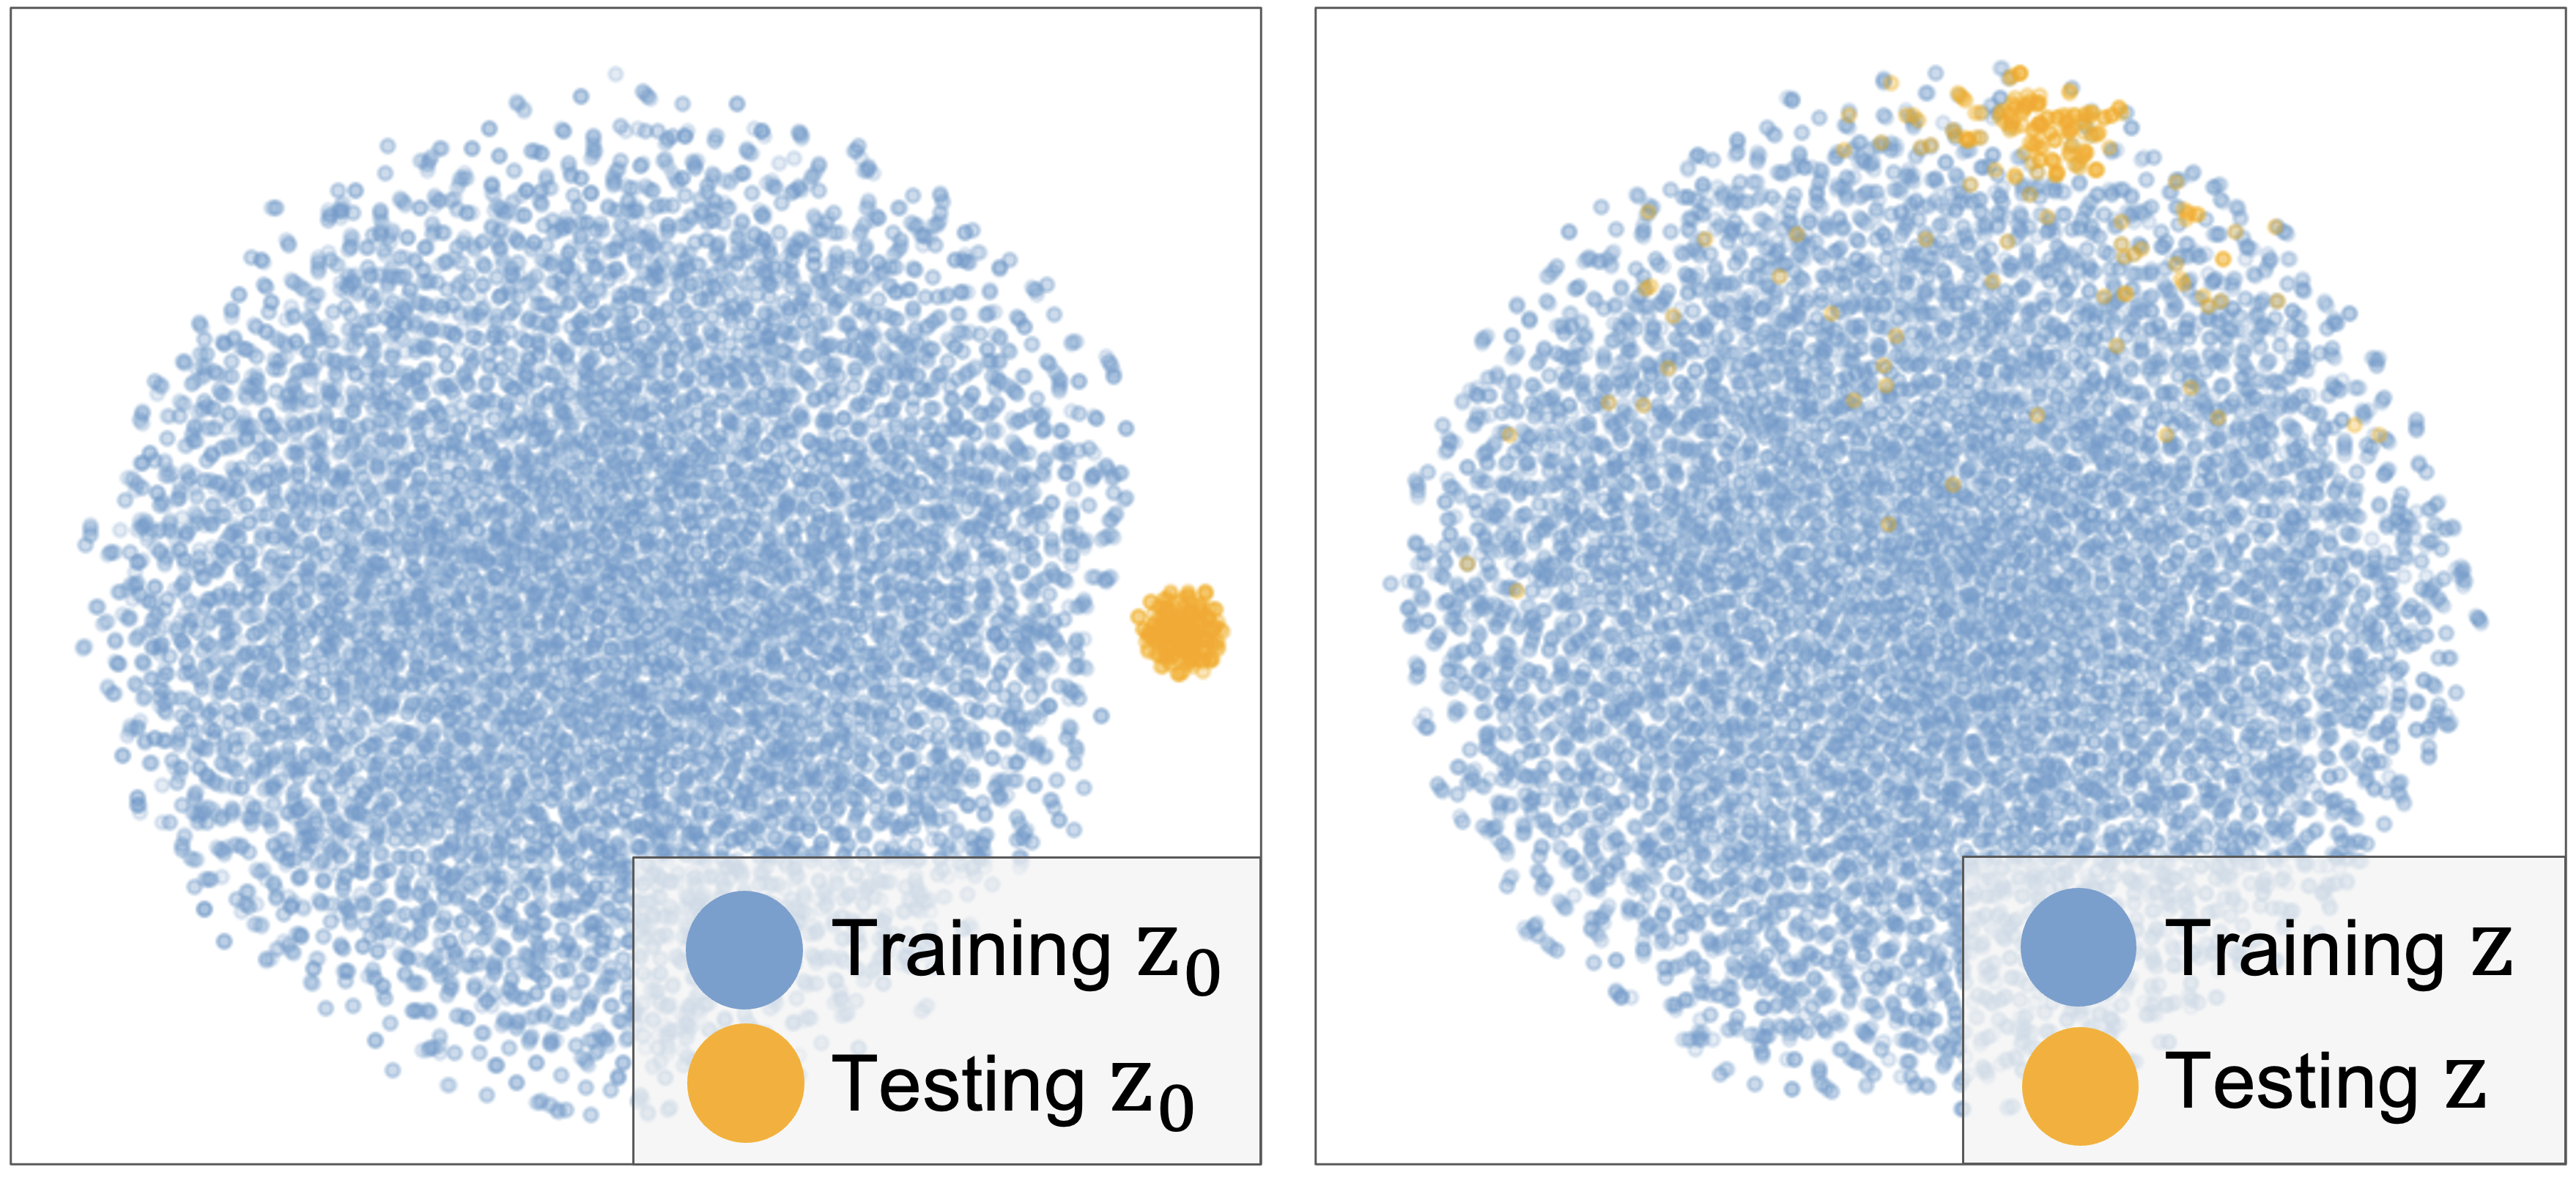
\includegraphics[width=\linewidth]{figures/tsne-all.png}
    \caption{t-SNE plot of latent variables in the Maze2D-medium. Left: Training $z_0$ from aggregated posterior $\E_{p_\mathcal{D}(\tau, y)}[p_\theta(z_0|\tau,y)]$. Testing $z_0$ from $p_\theta(z_0|y)$, disjoint from training population. Right: Distribution of $z=U_\alpha(z_0)$. }
    \label{fig:latent-tsne}
    \vspace{-2em}
\end{wrapfigure}


\cref{fig:maze2d_traj} visualizes samples from the training data and successful trajectories in testing. The left panels show that trajectories in training are suboptimal in terms of (1) being short in length and (2) containing very few goal-reaching instances. Trajectories on the right are generated by $10$ random runs with LPT, where the agent successfully navigates to the end goal from random starting positions in an effective manner. This indicates that the agent can discover the correlation between different $y$s to facilitate such stitching. 

To probe into the agent's understanding of trajectories' returns, we visualize the representation space of the latent variables. The left of \cref{fig:latent-tsne} is the aggregated posterior distribution of $z_0$. We can see that $z_0$ infered from $p_\theta(z_0|y)$ are distant away from the training population. The agent understands they are not very likely in the training set. The right of \cref{fig:latent-tsne} is the distribution of $z$, which is transformed from $z_0$ with the UNet, $z=U_\alpha(z_0)$. We observe that $z$s from the generated trajectories become ``in-distribution'' in the sense that some of them are mingled into the training population and the remaining lie inside a region coverable through linear interpolation of training samples. The agent understands what trajectories to generate even if they are unlikely among what it has seen. 




\subsection{Environment contingencies} 

To live in a stochastic world, contingent planning that is adaptable to unforeseen noises is desirable. \citet{paster2022you, yang2022dichotomy} discover that DT's performance would degrade in stochastic environments due to inevitable overfitting towards contingencies. We examine LPT and other baselines in Connect Four from~\citet{paster2022you}. Connect Four is a two-player game, where the opponent will make adversarial moves to deliberately disturb an agent's plan. According to the empirical study from~\citet{paster2022you}, the degradation of DT is more significant than in stochastic Gym tasks from~\citet{yang2022dichotomy}. As shown in Table \ref{table:connect4}, LPT achieves the highest score with minimal variance. The ESPER baseline is from~\citet{paster2022you}, which is very relevant to LPT as it is also a latent variable model. ESPER learns the latent variable model with an adversarial loss. It further adds a clustering loss in the latent space. LPT's on-par performance may justify that MLE upon a more flexible prior can play an equal role. 

\begin{table}[h]
% \vspace{-1.5em}
\centering
\caption{Evaluation results on Connect Four. \textbf{Bold} highlighting indicates top scores.}
\label{table:connect4}
\resizebox{0.65\linewidth}{!}{%
\centering
\begin{tabular}{lccccc}
\toprule
{Dataset}  &\multicolumn{1}{c}{CQL} & \multicolumn{1}{c}{DT} &\multicolumn{1}{c}{ESPER} &\multicolumn{1}{c}{LPT}\\
\midrule
Connect Four  &{$0.61\pm0.05$} &$0.8\pm0.07$ &$\mathbf{0.99}\pm0.03$ &$\mathbf{0.99}\pm0.01$\\
\bottomrule
% \bottomrule
\end{tabular}
}
\end{table}